\documentclass[11pt]{article}

\usepackage[margin=1in]{geometry}
\usepackage[authoryear,round]{natbib}
\usepackage{amsmath,amssymb}
\usepackage{booktabs}
\usepackage{array}
\usepackage{graphicx}
\usepackage{xcolor}
\usepackage{hyperref}
\IfFileExists{placeins.sty}{\usepackage{placeins}}{\newcommand{\FloatBarrier}{}}

\graphicspath{{figures/}}

\hypersetup{
  colorlinks=true,
  linkcolor=blue,
  citecolor=blue,
  urlcolor=blue
}

\newcommand{\modelname}{ESRL-FIMr1p1}
\newcommand{\modelshort}{FIMr1p1}
\newcommand{\methodname}{\modelshort{}-FlowMatch}
\newcommand{\stagenum}[1]{(\textbf{#1})}

\title{Physically Informed Stochastic Flow Matching for Global Probabilistic Subseasonal Forecast Refinement}
\author{Author Name(s)\\Affiliation\\\texttt{author@email.edu}}
\date{}

\begin{document}
\maketitle

\begin{abstract}
Skillful subseasonal forecasts of precipitation and near-surface temperature are needed for hydrologic risk, agriculture, energy planning, public health, and disaster preparedness, yet raw dynamical ensembles retain regional biases and imperfect probabilistic calibration at weeks 1--4. We introduce \methodname{}, a global machine-learning framework that refines \modelname{} (\modelshort{}) subseasonal ensemble guidance into stochastic, spatially coherent ensemble forecasts of weekly precipitation and 2\,m temperature. The central design choice is to generate ensemble members from a physically informed stochastic prior rather than from isotropic Gaussian noise: initial perturbations combine EOF structures conditioned on MJO, NAO, ENSO, and lead-week state with random support and variance-tempered spread control. A lead-aware flow-matching U-Net is conditioned on \modelshort{} ensemble summary statistics, recent observed land--ocean--atmosphere predictors, static geography, seasonal phase, and lead time; it predicts precipitation directly and 2\,m temperature as a residual relative to the target-lead \modelshort{} ensemble mean. Because probabilistic members are produced by integrating the learned velocity field from these structured initial states, the flow refines physically plausible large-scale covariance patterns instead of constructing all spatial organization from white noise. On the held-out 2021--2023 evaluation, \methodname{} reduces all-case CRPS relative to raw \modelshort{} by 32.2\% for precipitation and 34.0\% for 2\,m temperature globally, with comparable land-only gains (32.3\% and 32.7\%) and positive CRPS and RMSE skill in every season--lead cell. A controlled ablation isolates the contribution of the prior itself: at fixed checkpoint, ensemble size, and ODE solver, replacing Gaussian initialization with the regime-conditioned EOF prior improves precipitation CRPS skill from 24.9\% to 28.4\% and temperature CRPS skill from 41.7\% to 43.2\%. Skill extends to the tails: on an observed-95th-percentile event subset, CRPS improves by 13.8\% (precipitation) and 26.8\% (temperature), calibrated Brier skill gains are positive for both variables, and case studies of the July 2022 UK heatwave and January 2023 California atmospheric-river sequence show sharper, better-placed tail probabilities at multi-week lead.
\end{abstract}

\section{Introduction}
\label{sec:intro}

Subseasonal-to-seasonal (S2S) prediction occupies the difficult interval between deterministic weather prediction and seasonal climate outlooks, sometimes described as a predictability valley. At this range, atmospheric initial conditions lose deterministic control while slower land, ocean, and tropical modes can still provide useful predictability \citep{Vitart2017,RobertsonVitart2018}. Forecast users nevertheless need calibrated probabilities rather than a single best estimate, especially for precipitation and temperature extremes whose societal consequences depend on tail risk. This motivates methods that use physically based dynamical guidance while correcting systematic forecast errors and quantifying residual uncertainty.

\modelshort{} subseasonal forecasts provide a physically grounded ensemble prior but, like other dynamical S2S systems, contain flow-dependent bias, regional calibration errors, under- and overdispersion, and limited precipitation sharpness at longer leads. Statistical postprocessing and ensemble model output statistics have long been used to improve weather forecasts \citep{Gneiting2005,RaspLerch2018,Gronquist2021}, but gridpoint-oriented corrections struggle to preserve spatial coherence and cross-variable dependence without an explicit spatial model. Recent machine-learning weather models show that learned global forecast mappings can be highly skillful \citep{Bi2023,Lam2023}, and stochastic neural forecasts increasingly emphasize ensemble distributions and proper scoring rules rather than deterministic trajectory error alone \citep{Lang2024}. For subseasonal impacts, however, a useful system should neither discard dynamical model information nor evaluate rare events only through an ensemble mean.

We frame the problem as probabilistic forecast refinement. \modelshort{} supplies the dynamical forecast state; observed ocean, land, circulation, moisture, and MJO-related predictors supply recent boundary and large-scale context; static geography supplies persistent spatial structure; and a flow-matching model learns an observation-consistent distribution over weekly precipitation and 2\,m temperature. Flow matching trains continuous generative models by regressing velocity fields along probability paths \citep{Lipman2023,Liu2023}, making it a natural fit for stochastic ensemble generation when paired with climate-informed initial perturbations. In this setting the ensemble noise is not a disposable implementation detail: it defines the starting distribution of every forecast member and therefore controls which spatial covariance structures the learned velocity field must refine.

The contributions are fourfold. First, we formulate a global $1^\circ$ weekly S2S forecast-refinement task for precipitation and 2\,m temperature conditioned on \modelshort{} ensemble summaries. Second, we implement a lead-aware multi-target flow-matching architecture with static geography, global-context cross-attention, separate precipitation and temperature heads, and structured velocity losses, reducing competition between short-lead synoptic corrections and longer-lead planetary-scale behavior. Third, we introduce a physically informed stochastic ensemble prior: EOF perturbations conditioned on MJO, NAO, ENSO, and lead week are blended with random support and variance-tempered spread adjustment, and the same structured-noise family is used during training and inference to avoid prior mismatch. Fourth, we evaluate routine skill, the stochastic prior, and high-impact extremes as related but distinct verification problems, using CRPS, RMSE, bias, correlation, raw and reliability-calibrated Brier skill scores, season--lead matrices, spatial skill maps, observed-threshold event subsets, and named-event tail diagnostics.

\begin{figure}[t]
\centering
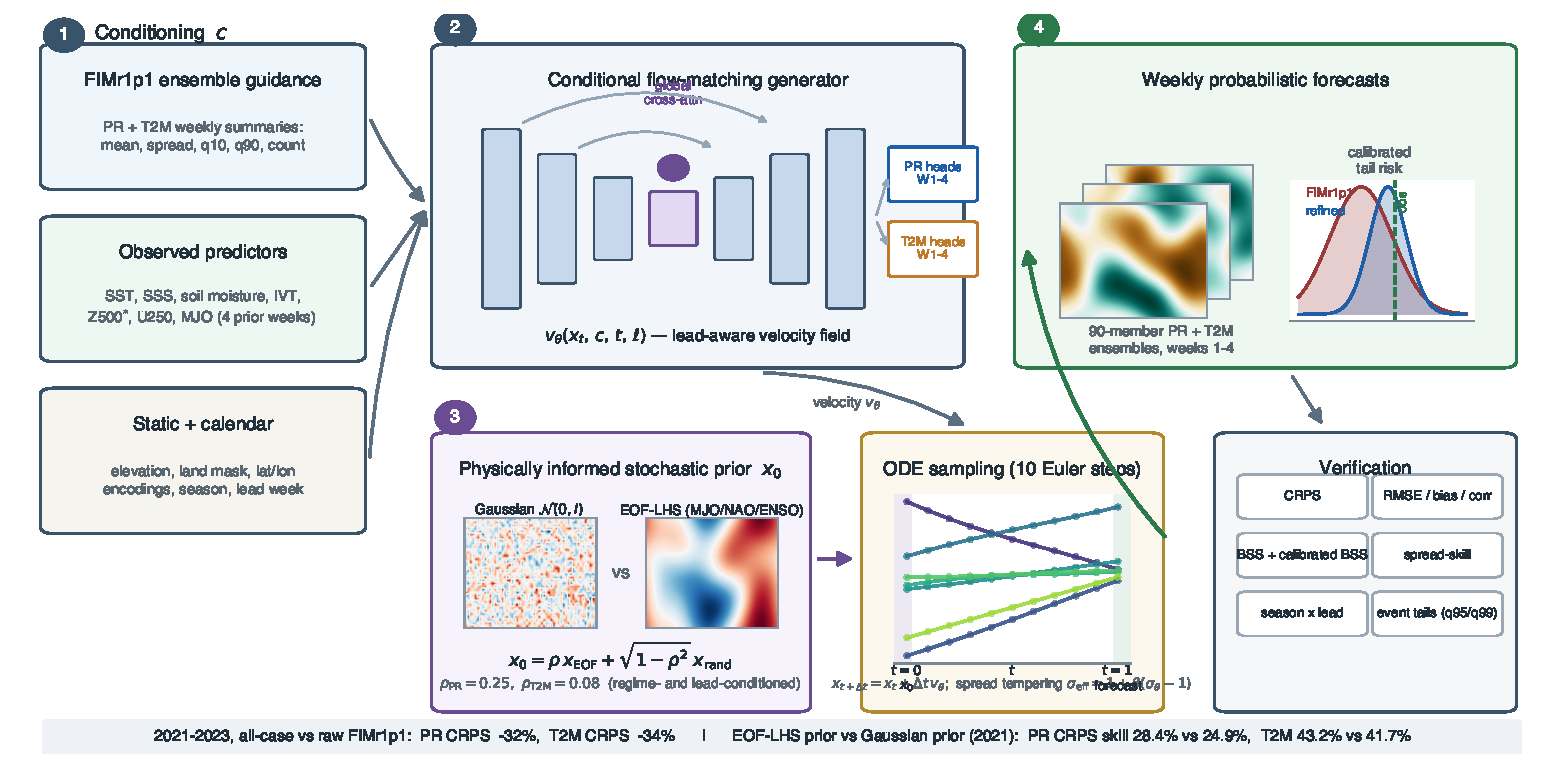
\includegraphics[width=\linewidth]{fig1_framework_overview}
\caption{The \methodname{} forecast-refinement framework. \stagenum{1} \modelshort{} ensemble summaries, recent observed predictors, and static/calendar fields form the conditioning tensor $c$. \stagenum{2} A lead-aware flow-matching U-Net with global-context cross-attention and separate precipitation/temperature heads learns the conditional velocity field $v_\theta(x_t,c,t,\ell)$. \stagenum{3} Ensemble members are initialized from a physically informed stochastic prior---regime-conditioned EOF-LHS perturbations blended with Gaussian support ($x_0=\rho\,x_{\mathrm{EOF}}+\sqrt{1-\rho^2}\,x_{\mathrm{rand}}$)---and integrated to $t{=}1$ with ten Euler steps under variance-tempered spread control. \stagenum{4} The result is a 90-member weekly precipitation and 2\,m temperature ensemble verified with all-case, spatial, calibration, and event-tail diagnostics. The two rendered noise fields contrast the isotropic Gaussian prior with the spatially coherent EOF-LHS prior that the ablation in Sect.~\ref{sec:results-noise} shows is responsible for part of the CRPS gain.}
\label{fig:overview}
\end{figure}

\section{Data and Forecast Problem}
\label{sec:data}

\subsection{Prediction task}

The prediction task is global weekly subseasonal forecasting on a $181\times360$ latitude--longitude grid. For each \modelshort{} initialization the system forecasts four weekly leads. The target variables are weekly mean precipitation, verified against GPCP-derived precipitation \citep{Adler2003}, and weekly mean 2\,m temperature, verified against ERA5-derived temperature \citep{Hersbach2020}. Precipitation is predicted in physical units after a square-root target transform. Temperature is represented during training as the residual between observed ERA5 2\,m temperature and the target-lead \modelshort{} ensemble-mean 2\,m temperature; the residual is added back to \modelshort{} at inference. Training uses 1999--2020; all results reported here are computed on the held-out 2021--2023 period from a single frozen checkpoint and a frozen generated-forecast archive.

\subsection{Dynamical and observed predictors}

The model conditions on \modelname{} weekly ensemble information for precipitation and 2\,m temperature. \modelname{} denotes the NOAA/ESRL FIMr1p1 forecast system in the S2S archive \citep{Vitart2017}, a finite-volume atmospheric model coupled with ocean and land components; the FIM model family is documented as a flow-following finite-volume global model \citep{Lee2006FIM}, and the surrounding NOAA numerical weather prediction context is summarized by \citet{Benjamin2019NWP}. Rather than passing only an ensemble mean, the system ingests five \modelshort{} summary statistics for each variable and lead: mean, standard deviation, 10th percentile, 90th percentile, and member count. Only the statistics for the target lead are used, which keeps the conditioning compact and aligns the correction with the verification lead.

Observed predictors are grouped into local target-grid predictors and global context predictors, each represented as four weekly pre-initialization fields. Local predictors are soil moisture and an MJO wave field; global context predictors are sea-surface temperature, sea-surface salinity, integrated vapor transport, 500\,hPa geopotential-height zonal deviation, and 250\,hPa zonal wind. Data sources are NOAA OISST sea-surface temperature \citep{Reynolds2007}, Copernicus sea-surface salinity \citep{CopernicusMarineSSS}, C3S/ESA soil moisture \citep{Dorigo2017}, and ERA5-derived circulation and moisture fields \citep{Hersbach2020}.

\subsection{Static geography}

Five static channels provide persistent spatial context: min--max-normalized elevation (GTOPO30-derived), a land mask, normalized latitude, and sine/cosine longitude. These allow the neural correction to depend on coastlines, orography, land--ocean contrast, and periodic longitude structure without relearning them from dynamic predictors. Table~\ref{tab:data-config} summarizes the full configuration.

\begin{table}[t]
\centering
\caption{Data and experiment configuration.}
\label{tab:data-config}
\small
\begin{tabular}{>{\raggedright\arraybackslash}p{0.30\linewidth}>{\raggedright\arraybackslash}p{0.62\linewidth}}
\toprule
Item & Configuration \\
\midrule
Target grid & Global $181\times360$, $1^\circ$ resolution \\
Forecast leads & Four weekly leads, weeks 1--4 \\
Targets & GPCP precipitation; ERA5 2\,m temperature residual relative to \modelshort{} ensemble mean \\
Dynamical input & \modelshort{} PR and T2M ensemble summaries: mean, standard deviation, q10, q90, member count \\
Observed local predictors & Soil moisture and MJO wave fields, four pre-initialization weeks \\
Observed global context & SST, SSS, IVT, Z500 zonal deviation, U250, four pre-initialization weeks \\
Static inputs & Elevation, land mask, normalized latitude, sine/cosine longitude \\
Training years & 1999--2020 \\
Evaluation years & 2021--2023 (held out) \\
Test ensemble & 90 generated members, 10 Euler steps \\
Ensemble prior & MJO/NAO/ENSO- and lead-conditioned EOF-LHS perturbations blended with Gaussian support; variance-tempered spread at inference \\
\bottomrule
\end{tabular}
\end{table}

\section{Method}
\label{sec:method}

\subsection{Forecast refinement view}

Let $y_{\ell}$ denote the observed weekly target field at lead week $\ell\in\{1,2,3,4\}$ and let $g_{\ell}$ denote the \modelshort{} ensemble information for the same lead. The goal is not to replace \modelshort{} with a free-running neural forecast but to learn a conditional forecast distribution
\begin{equation}
  p_{\theta}(y_{\ell}\mid g_{\ell}, z, s, \ell),
\end{equation}
where $z$ contains recent observed predictors and $s$ contains static geography and calendar information. The dynamical model provides a physically informed prior state; machine learning provides spatially coherent, observation-consistent distributional corrections.

\subsection{Conditional flow matching}

Let $x_1$ be the normalized target field and $x_0$ a stochastic initial field. For $t\in[0,1]$ the model is trained on the linear path
\begin{equation}
  x_t = t\,x_1 + (1-t)\,x_0,
\qquad
  v^\star = x_1 - x_0 .
\end{equation}
The network predicts $v_{\theta}(x_t,c,t,\ell)$, where $c$ is the conditioning tensor. The base velocity objective is
\begin{equation}
  \mathcal{L}_{\mathrm{vel}} =
  \frac{1}{N}\sum_i w_{\mathrm{area},i}\, w_{\mathrm{lead},i}
  \left\lVert v_{\theta}(x_t,c,t,\ell)_i - v^\star_i \right\rVert_2^2,
\end{equation}
where $w_{\mathrm{area}}$ is a latitude-cosine area weight and $w_{\mathrm{lead}}$ increases from week~1 to week~4 as $(1.0,\,1.2,\,1.5,\,2.0)$, reflecting the greater difficulty and user value of long-lead corrections. Forecast samples are generated by explicit Euler integration,
\begin{equation}
  x_{t+\Delta t} = x_t + \Delta t\, v_{\theta}(x_t,c,t,\ell),
\end{equation}
from $t=0$ to $t=1$ in 10 steps; the test configuration draws 90 ensemble members.

\subsection{Architecture}

The velocity model wraps a U-Net backbone \citep{Ronneberger2015} in the flow-matching formulation (Fig.~\ref{fig:overview}, stage~2). The state channels are the precipitation and 2\,m temperature residual/target fields; conditioning channels are concatenated with the flow state, and static geography is appended internally. A context MLP summarizes the conditioning tensor through spatial means and standard deviations, lead week is represented by a learned embedding, and a global-context encoder maps coarse global predictor fields into spatial tokens. A bottleneck cross-attention module lets local U-Net bottleneck cells attend to these global tokens, giving each grid cell access to planetary-scale teleconnection information at low cost.

The output stage contains separate lead-specific precipitation and temperature heads, plus separate variance heads for each variable and lead. This shares most spatial representation learning while allowing week-1 and week-4 corrections to specialize, avoiding capacity competition between filters that correct short-lead weather-scale errors and filters that represent slower week-3/4 circulation. It also avoids forcing precipitation and temperature---which have very different spatial and distributional structure---through a single final projection.

\subsection{Target transforms and physical bounds}

Precipitation is square-root transformed before normalization and decoded by squaring, with a nonnegative clamp; this compresses the dynamic range of heavy precipitation and prevents negative rain at inference. Temperature is trained as a \modelshort{} residual bounded by global statistics and added back to the target-lead \modelshort{} ensemble mean at decode time. These transformations are not conservation constraints, but they impose simple physical bounds that keep generated samples meteorologically plausible.

\subsection{Structured velocity loss}

The velocity loss is augmented with variable-specific spatial-structure terms: a pixel loss, first-gradient losses in latitude and longitude, and coarse losses after $2\times$ and $4\times$ average pooling,
\begin{equation}
  \mathcal{L}_{q} =
  \mathcal{L}_{\mathrm{pix},q}
  + \lambda_{\nabla,q}\mathcal{L}_{\nabla,q}
  + \lambda_{2,q}\mathcal{L}_{2,q}
  + \lambda_{4,q}\mathcal{L}_{4,q},
  \qquad q\in\{\mathrm{PR},\mathrm{T2M}\},
\end{equation}
with the final loss averaging the two per-variable totals. This encourages the learned velocity field to preserve both local gradients and broader spatial organization.

\subsection{Physically informed stochastic prior}
\label{sec:method-prior}

The stochastic forecast distribution begins with the initial field $x_0$. In a conventional generative forecast $x_0$ is drawn from independent Gaussian noise---mathematically convenient, but it asks the learned velocity field to create all coherent precipitation and temperature structure during the ODE integration. For subseasonal prediction this is an unnecessarily weak prior, because large-scale modes already constrain plausible spatial covariance. \methodname{} therefore treats the ensemble perturbation itself as a physical input to the forecast system.

EOF perturbations are conditioned on MJO, NAO, ENSO, and lead-week state when the corresponding bases are available. The MJO is a known source of subseasonal tropical and extratropical predictability \citep{MaddenJulian1971,WheelerHendon2004}; NAO and ENSO states provide additional large-scale circulation and oceanic regime information \citep{WallaceGutzler1981,BarnstonLivezey1987}; EOF bases compactly represent recurring spatial modes \citep{Lorenz1956}. Latin-hypercube sampling (LHS) within the EOF coefficient space makes a finite ensemble explore the structured perturbation distribution more evenly than repeated independent draws. For each variable $q$ the structured and random components are blended as
\begin{equation}
  x_0^{(q)} = \rho_q\, x_{\mathrm{EOF}}^{(q)} + \sqrt{1-\rho_q^2}\; x_{\mathrm{rand}}^{(q)},
\end{equation}
with $\rho_{\mathrm{PR}}=0.25$ and $\rho_{\mathrm{T2M}}=0.08$ at evaluation time (ramped from 0.15 and 0.05 during early training). Precipitation deliberately receives the stronger structured prior, reflecting the greater importance of organized tropical convection, monsoon structure, and spatial displacement uncertainty for weekly precipitation.

Using structured noise only at inference would expose the ODE solver to initial states the velocity model never saw during training. Training therefore uses the same EOF-LHS mixture, so the learned flow matches the sampling path used at evaluation: the initial state already contains broad spatial covariance, and the velocity field can focus on observation-conditioned refinement rather than constructing planetary-scale structure from white noise. The decisive test is not ``more ensemble members'' but whether a physically informed prior improves CRPS and tail probabilities relative to a pure Gaussian prior at the same checkpoint, ensemble size, and ODE-step count (Sect.~\ref{sec:results-noise}).

\subsection{Variance-tempered spread control}

Variance heads estimate a relative spread multiplier $\sigma_\theta$ trained against a normalized absolute velocity residual and regularized toward a physically moderate range. At inference the multiplier is clipped, coarse-grained over an 8-grid-cell kernel, and tempered toward one,
\begin{equation}
  \sigma_{\mathrm{eff}} = 1 + \beta_q(\sigma_{\theta}-1),
\end{equation}
with $\beta_{\mathrm{PR}}=0.45$ and $\beta_{\mathrm{T2M}}=0.03$. This lets the ensemble express heteroscedastic uncertainty without allowing the variance pathway to dominate the flow trajectory.

\FloatBarrier

\section{Experimental Design}
\label{sec:design}

\subsection{Training configuration}

The production configuration trains from scratch with batch size 4, learning rate $2\times10^{-5}$, weight decay $10^{-4}$, BF16 mixed precision, and an 80-epoch horizon organized into three phases: epochs 1--25 emphasize the velocity field, epochs 26--54 enable joint velocity/variance learning, and epochs 55--80 train variance heads only. Context dropout is applied to non-\modelshort{} predictors during training, but \modelshort{} conditioning is always kept active because it is the operational dynamical prior. The flow-time sampler emphasizes low and middle interpolation times, increasing exposure to the early portion of the ODE trajectory where the stochastic initial condition most strongly shapes ensemble structure.

\subsection{Baseline}

The principal baseline is the raw \modelshort{} ensemble on the same variable, lead, initialization, and grid. For deterministic metrics the \modelshort{} ensemble mean is compared with the \methodname{} ensemble mean; for probabilistic metrics both ensembles are evaluated as empirical predictive distributions. This is the fairest comparison for a refinement system, because \modelshort{} is both the conditioning source and the operational forecast to be improved.

\subsection{Verification protocol}

The primary all-case probabilistic metric is the continuous ranked probability score \citep{MathesonWinkler1976,Hersbach2000,GneitingRaftery2007}. For an empirical ensemble $\{x_m\}_{m=1}^{M}$ and observation $y$,
\begin{equation}
  \mathrm{CRPS} =
  \frac{1}{M}\sum_{m=1}^{M}\lvert x_m-y\rvert
  - \frac{1}{2M^2}\sum_{m=1}^{M}\sum_{n=1}^{M}\lvert x_m-x_n\rvert .
\end{equation}
Deterministic metrics are ensemble-mean RMSE, MAE, bias, and Pearson correlation; all spatial reductions use latitude-cosine weights, and results are reported both on all grid points (``All'') and on a land mask (``Land''). Relative skill for a negatively oriented score $S$ is
\begin{equation}
  \mathrm{Skill}_{S} = 100\left(1 - \frac{S_{\mathrm{ML}}}{S_{\mathrm{FIM}}}\right).
\label{eq:skill}
\end{equation}

Extremes are evaluated as forecast-distribution problems rather than ensemble-mean reconstruction problems. Events are defined by observed monthly climatological threshold maps, with the default event $y \ge q_{0.95}$ at each grid cell and a minimum precipitation threshold of 5\,mm\,day$^{-1}$. For each event definition we compute raw and reliability-calibrated Brier scores and Brier skill scores \citep{Brier1950,Murphy1973}; the calibrated path uses leave-one-year-out logistic reliability calibration of raw exceedance probabilities. This separates two questions: whether the ensemble assigns high probability to observed extremes, and whether those probabilities are statistically reliable.

\subsection{Noise-prior ablation protocol}

Because \methodname{} is a stochastic generator, the ensemble initialization must be evaluated as a first-order algorithmic choice. We compare sampling strategies at the same checkpoint, data split, ensemble size, ODE solver, and conditioning fields, changing only the initial prior: (i) pure Gaussian, $x_0\sim\mathcal{N}(0,I)$, which tests the learned flow without physical covariance in the initial ensemble, and (ii) the production physically informed prior, combining regime-conditioned EOF-LHS perturbations with variance-tempered spread control. The primary ablation score is CRPS skill relative to raw \modelshort{} (Eq.~\ref{eq:skill}); a secondary score is the relative CRPS reduction versus the Gaussian neural ensemble, which isolates the value of the physical prior after the architecture and dynamical conditioning are held fixed.

\subsection{Named extreme-event case studies}

Two high-impact cases with different variables, regions, and dynamical drivers are examined in the main text (Table~\ref{tab:event-definitions}): the July 2022 UK heatwave, during which the UK record high of 40.3\,$^\circ$C at Coningsby was verified by the Met Office \citep{MetOffice2022Heatwave}, and the December 2022--January 2023 California atmospheric-river storm sequence \citep{CW3E2023CaliforniaAR}. A third precipitation case, the June 2022 northeastern Bangladesh/Sylhet floods \citep{Reuters2022BangladeshFloods}, is provided in the supplement. For each case, verification uses the initialization whose week-4 target week overlaps the event window---the hardest and most valuable subseasonal setting---with maps of ensemble upper quantiles, event CRPS, and event BSS.

\begin{table}[t]
\centering
\caption{Named extreme-event case definitions.}
\label{tab:event-definitions}
\small
\begin{tabular}{>{\raggedright\arraybackslash}p{0.26\linewidth}llp{0.22\linewidth}p{0.20\linewidth}}
\toprule
Event & Variable & Valid window & Region & Verification focus \\
\midrule
UK heatwave & T2M & week of 18--19 Jul 2022 & UK / western Europe & hot-tail q95, event CRPS, BSS \\
California atmospheric rivers & PR & Jan 2023 storm week & California / U.S. West Coast & heavy-rain q95, event CRPS, BSS \\
Bangladesh/Sylhet flood (suppl.) & PR & 17--23 Jun 2022 & NE Bangladesh / Meghalaya & p95/p99 exceedance, event CRPS \\
\bottomrule
\end{tabular}
\end{table}

\FloatBarrier

\section{Results}
\label{sec:results}

All numerical results are computed from the frozen 2021--2023 matrix-evaluation products. ``All'' rows evaluate all grid points; ``Land'' rows use the land mask. Extreme-event scores use monthly local observed $q_{0.95}$ thresholds (precipitation additionally $\ge 5$\,mm\,day$^{-1}$), and calibrated BSS uses leave-one-year-out logistic reliability calibration.

\subsection{Overall skill}
\label{sec:results-overall}

Table~\ref{tab:headline-results} reports weighted aggregates across all valid-season and lead cells. \methodname{} improves every headline probabilistic and deterministic score for both variables and both masks: all-grid CRPS falls by 32.2\% for precipitation and 34.0\% for temperature, RMSE by 25.6\% and 22.4\%, and land-mask CRPS by 32.3\% and 32.7\%. Absolute bias is reduced strongly for precipitation (0.44 to 0.19\,mm\,day$^{-1}$ all-grid) and for land temperature ($-0.31$ to 0.13\,K); the single degradation is all-grid temperature bias, which grows from a very small 0.04\,K to a still-small 0.14\,K---an acceptable trade against the large CRPS and RMSE gains, but one we report explicitly. Pattern correlation increases for both targets (precipitation 0.576 to 0.711 all-grid, 0.603 to 0.745 land; temperature 0.989 to 0.993 and 0.987 to 0.992). Calibrated BSS gains are positive for precipitation in both masks ($+0.019$ all-grid, $+0.024$ land) and for land temperature ($+0.016$), with a marginally negative all-grid temperature value ($-0.004$) traceable to week~4 (Table~\ref{tab:lead-mask-results}).

\begin{table}[t]
\centering
\caption{Headline all-case skill on the held-out 2021--2023 evaluation. Positive change means \methodname{} improves on \modelshort{}; the bias rows report absolute-bias change. Units are mm\,day$^{-1}$ (PR) and K (T2M).}
\label{tab:headline-results}
\small
\begin{tabular}{lllrrr}
\toprule
Mask & Variable & Metric & \modelshort{} & \methodname{} & Change \\
\midrule
All & PR & CRPS & 1.591 & 1.079 & $+32.2\%$ \\
All & PR & RMSE & 3.448 & 2.565 & $+25.6\%$ \\
All & PR & $\lvert$Bias$\rvert$ & 0.437 & 0.192 & $+56.1\%$ \\
All & T2M & CRPS & 1.193 & 0.788 & $+34.0\%$ \\
All & T2M & RMSE & 2.239 & 1.738 & $+22.4\%$ \\
All & T2M & $\lvert$Bias$\rvert$ & 0.040 & 0.138 & $-248.3\%$ \\
Land & PR & CRPS & 1.302 & 0.881 & $+32.3\%$ \\
Land & PR & RMSE & 3.083 & 2.294 & $+25.6\%$ \\
Land & PR & $\lvert$Bias$\rvert$ & 0.257 & 0.204 & $+20.7\%$ \\
Land & T2M & CRPS & 1.936 & 1.303 & $+32.7\%$ \\
Land & T2M & RMSE & 3.212 & 2.584 & $+19.5\%$ \\
Land & T2M & $\lvert$Bias$\rvert$ & 0.307 & 0.128 & $+58.4\%$ \\
\bottomrule
\end{tabular}
\end{table}

Figures~\ref{fig:pr-skill} and \ref{fig:t2m-skill} resolve these aggregates by season, lead, and geography. Every one of the 16 season--lead cells is improved for both variables and both masks: all-grid precipitation CRPS skill ranges from 27.7\% to 40.3\% (land 27.3--39.7\%), and all-grid temperature CRPS skill from 23.7\% to 48.1\% (land 26.6--43.8\%). The spatial maps show that gains are geographically coherent rather than driven by a few regions: precipitation improvements are largest where raw \modelshort{} CRPS is largest (tropical convergence zones, monsoon regions, orographic coasts), and temperature improvements are broad over land with the strongest corrections in regions of known systematic bias.

\begin{figure}[t]
\centering
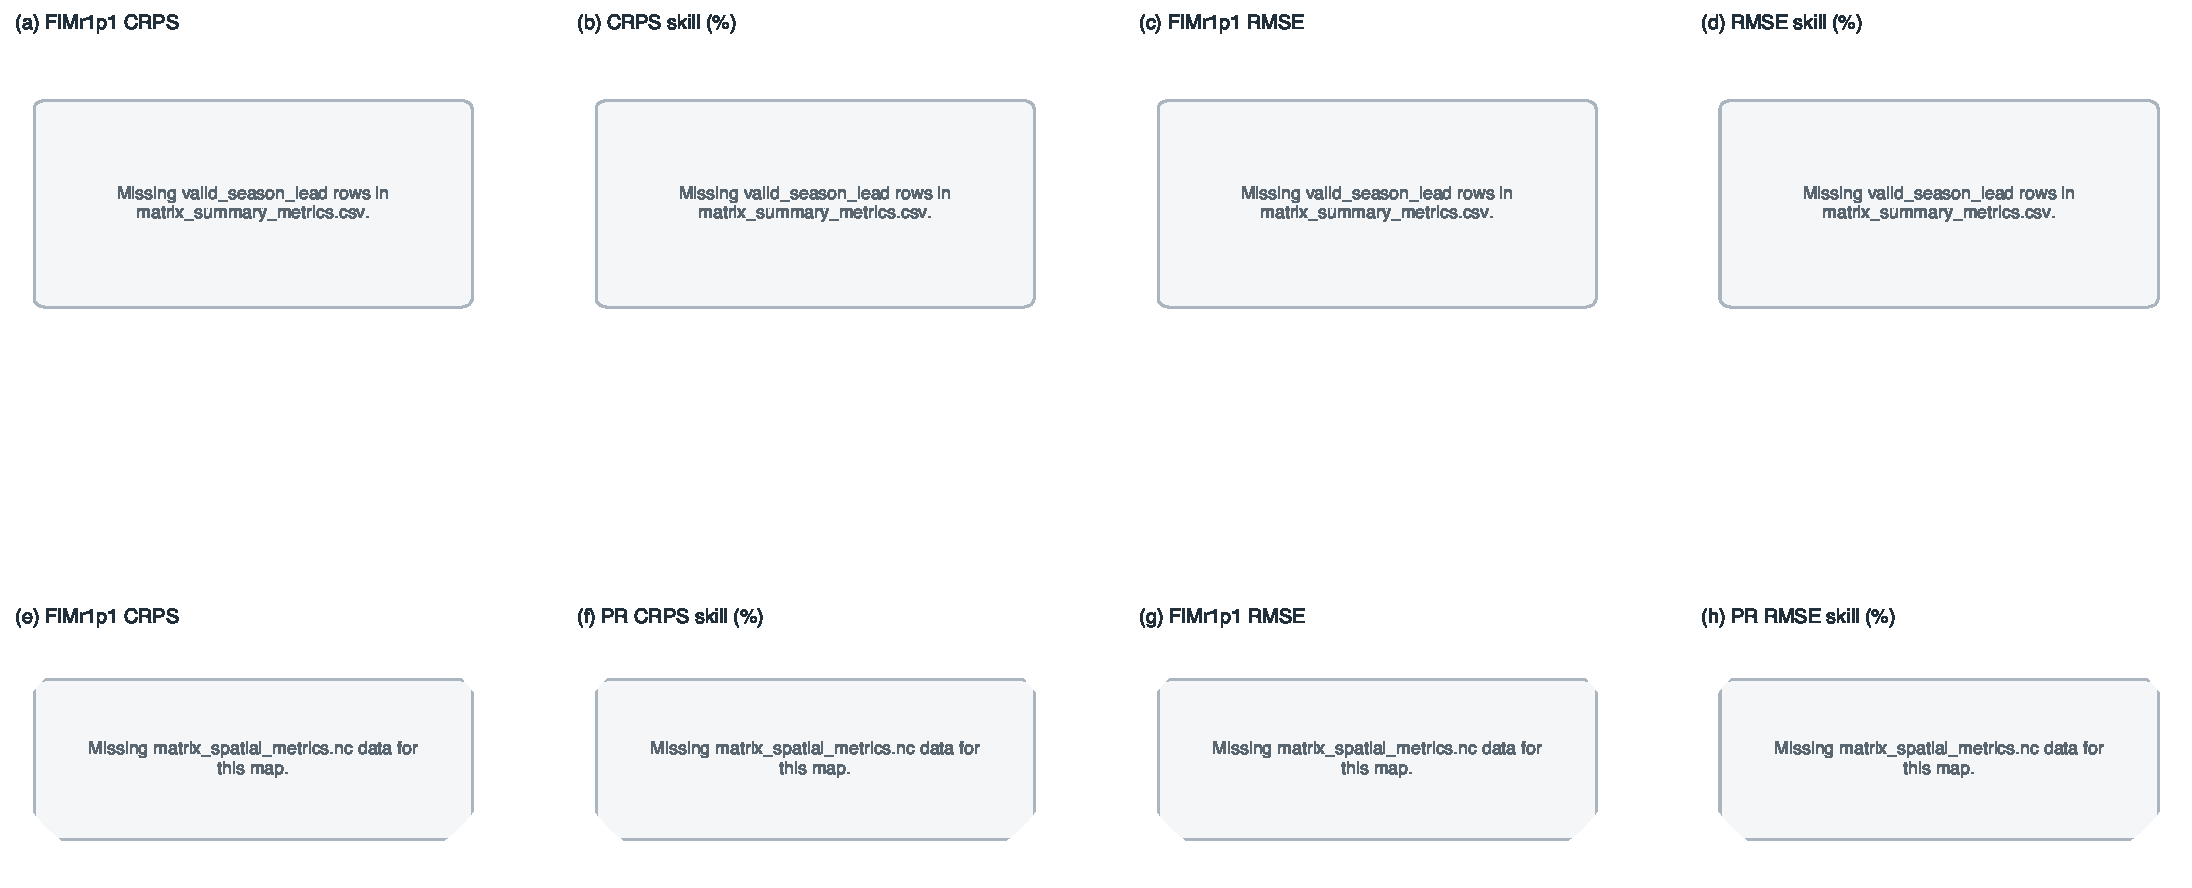
\includegraphics[width=\linewidth]{fig2_pr_skill}
\caption{Precipitation all-case skill versus \modelshort{}, 2021--2023. (a,~c) Season--lead matrices of raw \modelshort{} CRPS and RMSE; (b,~d) corresponding \methodname{} skill (\%, Eq.~\ref{eq:skill}) with the absolute \methodname{} score in parentheses; (e,~g) spatial maps of raw \modelshort{} CRPS and RMSE aggregated over seasons and leads; (f,~h) spatial maps of \methodname{} CRPS and RMSE skill. Blue denotes improvement over the dynamical baseline, red degradation.}
\label{fig:pr-skill}
\end{figure}

\begin{figure}[t]
\centering
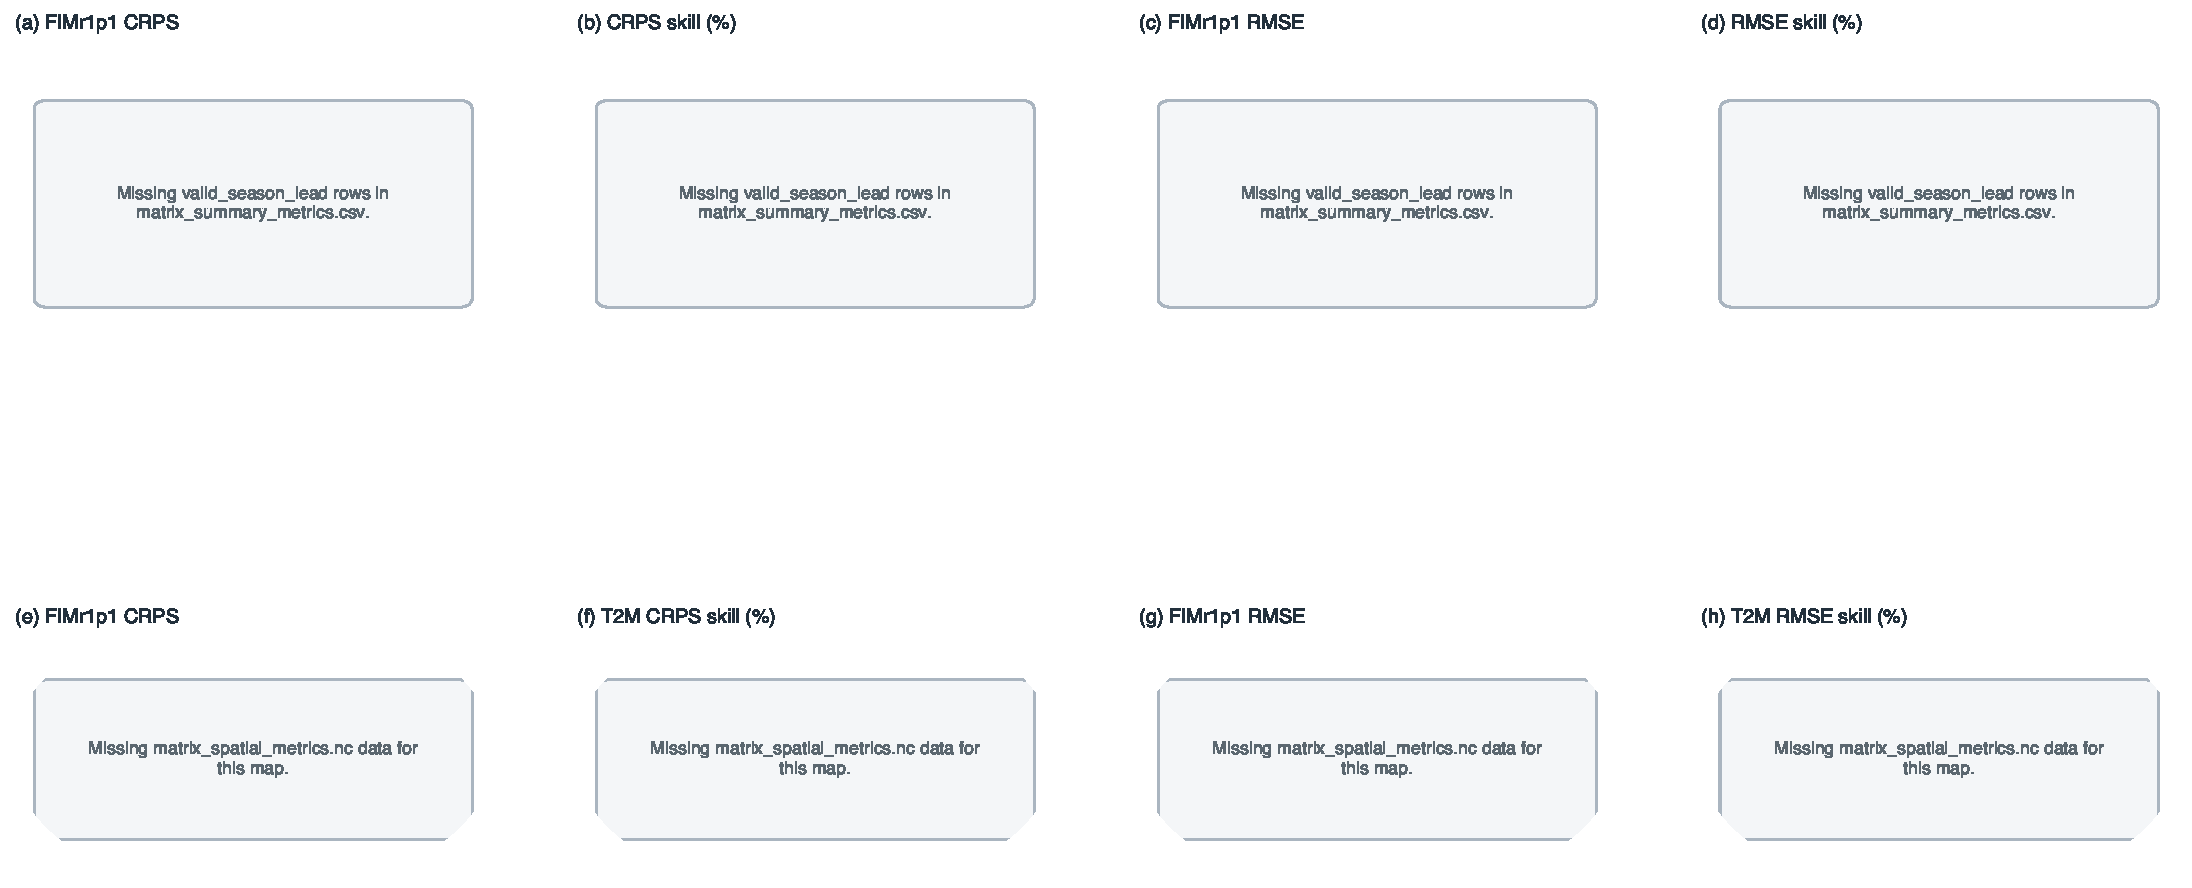
\includegraphics[width=\linewidth]{fig3_t2m_skill}
\caption{As in Fig.~\ref{fig:pr-skill}, but for 2\,m temperature.}
\label{fig:t2m-skill}
\end{figure}

Table~\ref{tab:lead-mask-results} shows the lead dependence. Skill is largest at week~1, where the correction problem is most deterministic, but remains large and stable through weeks 2--4 (all-grid precipitation CRPS skill 38.1\%, 31.7\%, 30.2\%, 29.5\%), indicating that the system is not merely a short-lead bias corrector: the week-3/4 gains are the operationally interesting result. Calibrated BSS gains are positive at all leads for precipitation and at weeks 1--3 for temperature, with a small negative all-grid week-4 temperature value ($-0.025$).

\begin{table}[t]
\centering
\caption{Lead-dependent all-case skill aggregated over valid seasons. CRPS and RMSE entries are percent improvements over \modelshort{} (Eq.~\ref{eq:skill}); calibrated BSS entries are \methodname{} minus \modelshort{}.}
\label{tab:lead-mask-results}
\small
\begin{tabular}{lllrrrr}
\toprule
Mask & Variable & Quantity & Week 1 & Week 2 & Week 3 & Week 4 \\
\midrule
All & PR & CRPS skill (\%) & 38.1 & 31.7 & 30.2 & 29.5 \\
All & PR & RMSE skill (\%) & 30.2 & 25.4 & 24.1 & 23.2 \\
All & PR & Cal.\ BSS gain & 0.046 & 0.011 & 0.009 & 0.009 \\
All & T2M & CRPS skill (\%) & 41.5 & 34.8 & 34.0 & 27.7 \\
All & T2M & RMSE skill (\%) & 25.5 & 22.0 & 22.4 & 20.8 \\
All & T2M & Cal.\ BSS gain & 0.002 & 0.004 & 0.003 & $-0.025$ \\
Land & PR & CRPS skill (\%) & 38.1 & 32.1 & 30.2 & 29.0 \\
Land & PR & RMSE skill (\%) & 29.9 & 26.1 & 24.2 & 22.5 \\
Land & PR & Cal.\ BSS gain & 0.045 & 0.019 & 0.016 & 0.015 \\
Land & T2M & CRPS skill (\%) & 40.1 & 32.3 & 31.0 & 29.6 \\
Land & T2M & RMSE skill (\%) & 23.8 & 18.0 & 18.7 & 19.0 \\
Land & T2M & Cal.\ BSS gain & 0.047 & 0.012 & 0.009 & $-0.005$ \\
\bottomrule
\end{tabular}
\end{table}

\subsection{Value of the physically informed prior}
\label{sec:results-noise}

The headline scores evaluate the full production system but do not identify how much skill comes from the stochastic prior itself. Figure~\ref{fig:noise-ablation} and Table~\ref{tab:noise-prior-ablation} therefore report the controlled ablation of Sect.~\ref{sec:design}: checkpoint, 2021 full-year validation data, ensemble size, ODE steps, and conditioning are fixed, and only the initial noise prior and spread tempering change.

Pure Gaussian sampling already improves substantially over raw \modelshort{} (precipitation CRPS skill 24.9\%, temperature 41.7\%), confirming that the conditional flow itself is a strong distributional corrector. Adding the regime-conditioned EOF-LHS prior improves precipitation CRPS skill to 28.4\% and temperature to 43.2\%---relative CRPS reductions of 4.7\% and 2.6\% versus the Gaussian neural ensemble. The interpretation is not that EOF perturbations are a different random seed: a Gaussian prior asks the flow to synthesize all spatial covariance from scratch, whereas the EOF-LHS prior starts each member on a low-dimensional manifold of historically observed, regime-consistent anomaly structures, and the larger benefit for precipitation is consistent with its greater sensitivity to displacement and organization uncertainty.

\begin{figure}[t]
\centering
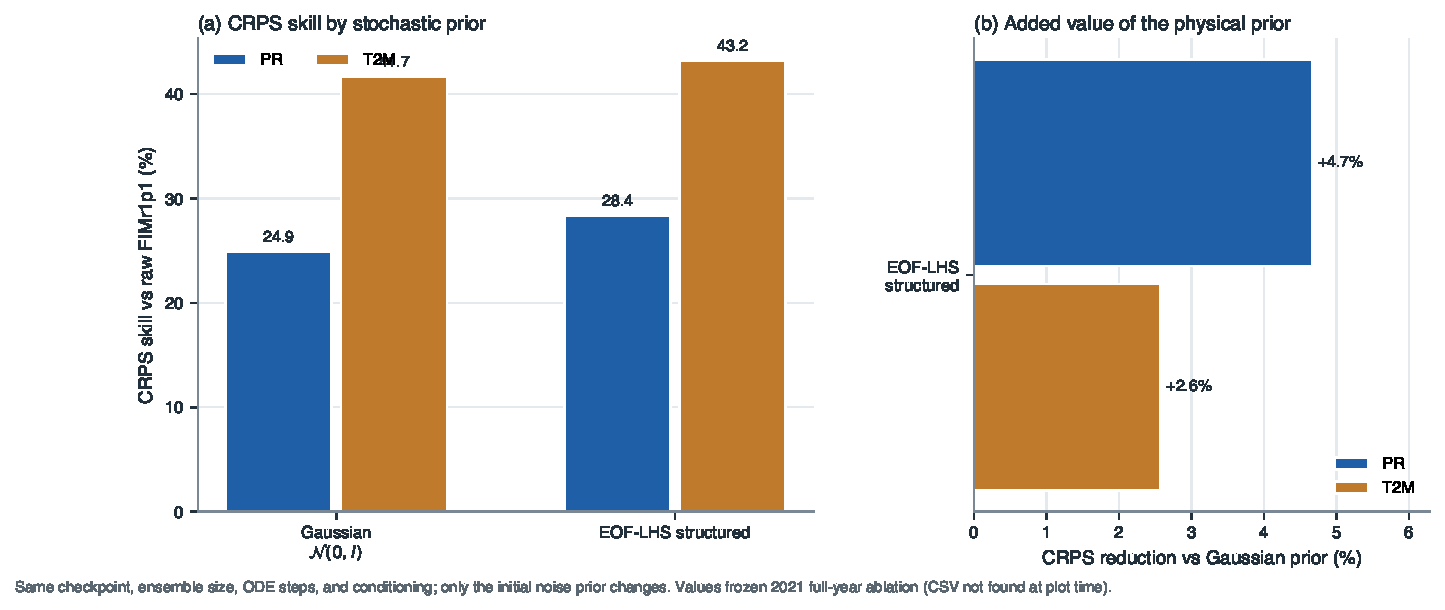
\includegraphics[width=0.92\linewidth]{fig4_noise_ablation}
\caption{Noise-prior ablation at fixed checkpoint, ensemble size, ODE solver, and conditioning (2021 full year). (a) All-grid CRPS skill versus raw \modelshort{} for the pure Gaussian prior and the regime-conditioned EOF-LHS prior, for precipitation and 2\,m temperature. (b) Relative CRPS reduction of the physically informed prior with respect to the Gaussian neural ensemble, isolating the contribution of the prior after architecture and dynamical conditioning are held fixed.}
\label{fig:noise-ablation}
\end{figure}

\begin{table}[t]
\centering
\caption{Noise-prior ablation, all-grid CRPS skill (\%) versus raw \modelshort{} (2021 full year, 52 batches). The EOF-based setting uses the higher-spread regime-conditioned EOF-LHS configuration ($\rho_{\mathrm{PR}}=0.25$, $\rho_{\mathrm{T2M}}=0.08$; $\beta_{\mathrm{PR}}=0.45$, $\beta_{\mathrm{T2M}}=0.03$).}
\label{tab:noise-prior-ablation}
\small
\begin{tabular}{>{\raggedright\arraybackslash}p{0.34\linewidth}p{0.24\linewidth}rr}
\toprule
Strategy & Spread control & PR & T2M \\
\midrule
Raw \modelshort{} ensemble & native & 0.0 & 0.0 \\
Gaussian prior $\mathcal{N}(0,I)$ & none & 24.9 & 41.7 \\
EOF-LHS physically informed prior & variance-tempered & \textbf{28.4} & \textbf{43.2} \\
\bottomrule
\end{tabular}
\end{table}

\subsection{Skill on observed extremes}
\label{sec:results-extremes}

Figure~\ref{fig:extreme-skill} evaluates the observed-threshold extreme subset. CRPS gains are smaller than all-case gains---as expected, since the subset removes the easy cases---but remain positive at every lead for both variables: aggregate extreme-subset CRPS skill is 13.8\% for precipitation and 26.8\% for temperature on the all-grid mask, and 18.0\% and 27.1\% on land. Calibrated BSS gains on the same subset are positive for both variables and both masks ($+0.031$ all-grid PR, $+0.032$ all-grid T2M, $+0.044$ land PR, $+0.041$ land T2M). The logistic calibration fits show that raw exceedance probabilities are overconfident for both systems (slopes below one), but \methodname{} is consistently closer to reliable: for example, the all-grid precipitation mean slope is 0.39 versus 0.10 for \modelshort{}, and 0.44 versus 0.10 on land. The neural ensemble therefore does not achieve its all-case CRPS gains by hedging toward climatology at the expense of the tails.

\begin{figure}[t]
\centering

\includegraphics[width=0.92\linewidth]{fig5_extreme_skill}
\caption{Skill on the observed extreme-event subset (local monthly $q_{0.95}$ exceedances; precipitation additionally $\ge 5$\,mm\,day$^{-1}$). (a) CRPS and (b) RMSE skill versus \modelshort{} by lead week for precipitation (blue) and 2\,m temperature (orange). Open markers show the corresponding all-case skill for reference; the gap between bars and markers measures how much harder the tail problem is than the routine problem.}
\label{fig:extreme-skill}
\end{figure}

\subsection{High-impact event case studies}
\label{sec:results-events}

For individual high-impact events, the relevant question is whether the observed event lies plausibly inside the forecast distribution---not whether the ensemble mean reproduces the event amplitude, which no calibrated multi-week ensemble should. Figures~\ref{fig:event-pr} and \ref{fig:event-t2m} therefore compare ensemble upper quantiles, event CRPS, and event BSS for the two primary cases at week-4 lead.

For the January 2023 California atmospheric-river week (Fig.~\ref{fig:event-pr}), the \methodname{} 95th-percentile precipitation field concentrates heavy-rain risk along the coastal and Sierra Nevada orography where the observed maxima occurred, whereas the raw \modelshort{} q95 is weaker and more diffuse. Event-mask CRPS is reduced over most of the affected region, and BSS for local heavy-rain exceedance improves over the coastal mountains, with stippling marking areas of robust improvement.

For the July 2022 UK heatwave (Fig.~\ref{fig:event-t2m}), raw \modelshort{} q95 temperatures remain several kelvin too cool over England at week-4 lead, placing the observed values far in the forecast tail. The refined ensemble shifts and sharpens the hot tail so that the observed anomaly pattern---including the southeastern England maximum---falls within the plausible upper quantiles, reduces event CRPS over the region, and increases hot-event BSS over most of England and Wales. Both cases illustrate the intended behavior of the framework: the physically informed ensemble does not sharpen by collapsing spread but by relocating probability mass toward the observation-consistent tail.

\begin{figure}[t]
\centering

\includegraphics[width=\linewidth]{fig6_event_pr_california}
\caption{California atmospheric-river precipitation case study (January 2023 storm week, week-4 lead). (a) Observed weekly precipitation; (b,~c) \modelshort{} and \methodname{} ensemble 95th percentiles; (d,~e) event-week CRPS for each system and (f) the resulting CRPS skill (\%, blue = improvement, stippled where $>10\%$); (g,~h) heavy-rain exceedance BSS for each system and (i) the BSS gain ($\times100$, stippled where robust).}
\label{fig:event-pr}
\end{figure}

\begin{figure}[t]
\centering

\includegraphics[width=\linewidth]{fig7_event_t2m_uk_heatwave}
\caption{As in Fig.~\ref{fig:event-pr}, but for 2\,m temperature during the July 2022 UK heatwave week (week-4 lead).}
\label{fig:event-t2m}
\end{figure}

\FloatBarrier

\section{Discussion}
\label{sec:discussion}

The main scientific value of this framework is its hybrid interpretation. \modelshort{} supplies a dynamically consistent prior distribution, while the neural model learns a conditional transformation toward observations. This differs both from a purely data-driven rollout and from scalar bias correction: the network sees spatially complete \modelshort{} forecast summaries, recent observed environmental predictors, and static geography, and produces a new ensemble distribution whose spatial covariance is inherited jointly from the learned flow and from the physically informed stochastic prior.

Several design choices matter for the observed behavior. The \modelshort{}-residual target for temperature focuses learning on forecast error rather than the full seasonal temperature range, which is consistent with the very high temperature correlations and the strong land bias correction. Static geography lets the model learn persistent biases tied to coastlines, elevation, and land--ocean contrast. Global-context cross-attention gives local grid cells access to the large-scale predictors that carry most subseasonal predictability. Separate precipitation and temperature heads respect the fact that precipitation is intermittent and displacement-prone while temperature is smoother and more strongly tied to large-scale circulation. The physically informed prior addresses a different part of the problem: it improves the geometry of the starting ensemble before the neural ODE is integrated, giving members plausible large-scale anomaly structures to refine---the ablation shows this contributes measurably beyond the flow itself, most strongly for precipitation.

The extreme-event results must be interpreted with the logic of probability forecasting. At subseasonal leads a well-calibrated ensemble mean should be smoother than individual outcomes; that is a feature, not a failure. The correct verification question for rare events is whether the forecast distribution assigns elevated, spatially relevant probability to the event and whether the observed value falls within a plausible forecast tail. On both the systematic $q_{0.95}$ subset and the named case studies, \methodname{} improves on the raw dynamical ensemble under exactly these distribution-based criteria, while the reliability-slope analysis shows the improvement is not an artifact of overconfident probabilities.

\section{Limitations and Future Work}
\label{sec:limitations}

Four limitations qualify these results. First, the reported metrics do not yet carry confidence intervals; block-bootstrap intervals over initializations should accompany the headline and ablation scores. Second, the structured stochastic prior is partly heuristic: EOF bases and teleconnection regimes are physically motivated, but the mixture weights $\rho_q$ are manually configured rather than learned end to end. Third, the variance mechanism adjusts the initial spread only and does not inject stochasticity continuously along the ODE trajectory. Fourth, precipitation remains hardest at weeks 3--4, where heavy rainfall is intermittent, spatially displaced, and often tied to mesoscale or tropical-cyclone processes that are not deterministic targets at subseasonal lead; neighborhood-based event verification partially, but not fully, compensates.

Natural next ablations are no-\modelshort{}-conditioning, no-static-geography, no-global-cross-attention, variance tempering on/off, learned versus fixed EOF mixture weights, and absolute versus residual temperature targets. Longer-term extensions include learning the stochastic prior directly, training with differentiable CRPS in physical units, conservation-aware precipitation constraints, stochastic paths (SDE rather than ODE sampling), and extending the target set to circulation variables.

\section{Conclusion}
\label{sec:conclusion}

We presented \methodname{}, a physically informed stochastic flow-matching framework for global probabilistic subseasonal forecast refinement. The system combines \modelshort{} ensemble guidance, recent observed predictors, static geography, a lead-aware multi-target flow-matching architecture, regime-conditioned EOF-LHS stochastic initialization, and variance-tempered spread control to generate 90-member ensemble forecasts of weekly precipitation and 2\,m temperature. On held-out 2021--2023 data the framework improves CRPS by roughly a third for both variables, with positive skill in every season--lead cell, geographically coherent gains, improved tail-event CRPS and calibrated Brier skill, and clear added value in week-4 case studies of the 2022 UK heatwave and the 2023 California atmospheric rivers.

The central message is twofold: machine learning can act as an observation-consistent distributional correction of a physics-based subseasonal ensemble rather than a replacement for it, and the stochastic prior used to generate ensemble members should itself carry physical information---a controlled ablation attributes a measurable share of the probabilistic skill to the regime-conditioned prior alone.

\bibliographystyle{plainnat}
\bibliography{references}

\end{document}
